\documentclass[../main.tex]{subfiles}
\graphicspath{{\subfix{../figures/}}}
\begin{document}

\section{Systematic Uncertainties}
\label{sec:systs}
The systematic uncertanties relevant to this analysis are divided into three categories: (1) beam flux, (2) interaction modeling, and (3) detector response modeling.  Beam flux and interaction modeling uncertainties are evaluated through event reweighting using either a multisim, multisigma, or morph technique.  With each approach, parameters affecting the probability of an interaction occuring are varied in a number of ``universes''.  One thousand universes are employed in this analysis, each of which is used to assign weights to neutrino interactions in order to assess the impact of the parameter variations.  A covariance matrix then captures the uncertainty on binned reconstructed observables by comparing event counts across different universes and the central value sample:
\begin{equation}
    V_{ij} = \frac{1}{N} \sum_{k}^{N} (M_{i}^{k} - M_{i}^{CV}) (M_{j}^{k} - M_{j}^{CV})
\end{equation}
where $N$ is the number of universes, $M_{i}^{k}$ ($M_{j}^{k}$) is the measured event count for bin $i$ ($j$) in the $kth$ universe, and $M_{i}^{CV}$ ($M_{j}^{CV}$) is the measured event count for bin $i$ ($j$) in the central value universe.

Detector response modeling uncertainties are evaluated with a ``uni-sim'' technique, where elements of the detector response model are modified in dedicated variation samples.  For every bin of a reconstructed observable, the ratio of events in the variation sample to events in the central value sample is represented in a spline that varies according to the number of standard deviations away from the nominal detector model parameter.  The spline is then evaluated for every selected interaction in a configurable number of universes (10,000 by default) defined by randomly thrown standard deviations.  Covariance matrix construction then follows in a manner analogous to the many-universes approach described previously.

\subsection{Flux Uncertainties}
The BNB flux at ICARUS is based on predictions from the MiniBooNE collaboration, which used the Geant4 simulation tool kit to model the propagation of particles produced in proton beam-target interactions \cite{bnbflux}.  Treatment of flux uncertainties, which arise from sources like hadron production, hadronic secondary interactions within the beam target, and beam focusing, are handled with a many-universes technique.  The full set of beam flux uncertainties studied in this analysis are shown in Table \ref{Tab:fluxparameters}.

\begin{table}[H]
    \caption{Flux uncertainties for $\nu_{\mu}$ CC $\pi^{0}$ selection}
    \vspace{0.1cm}
    \centering
    \begin{tabular}{ c c c } 
    \hline
    Variation & Description & Uncertainty [\%] \\
    \hline
    kminus & $K^{-}$ production in beam target & 0.01 \\
    kplus & $K^{+}$ production in beam target & 0.63 \\
    kzero & $K^{0}$ production in beam target & 0.03 \\
    piminus & $\pi^{-}$ production in beam target & 0.16 \\
    piplus & $\pi^{+}$ production in beam target & 5.34 \\
    expskin & Current induced on surface of focusing horn & 6.26 \\
    horncurrent & Current pulsed through focusing horn & 0.79 \\
    nucleoninexsec & Nucleon inelastic re-scattering in beam target & 0.80 \\
    nucleonqexsec & Nucleon QE re-scattering in beam target & 2.48 \\
    nucleontotxsec & Nucleon total re-scattering in beam target & 0.70 \\
    pioninexsec & $\pi$ inelastic re-scattring in beam target & 1.29 \\
    pionqexsec & $\pi$ QE re-scattering in beam target & 0.86 \\
    piontotxsec & $\pi$ total re-scattering in beam target & 0.99 \\
    \hline
    Total & & 8.91 \\
    \hline
    \end{tabular}
    \label{Tab:fluxparameters}
\end{table}

\subsection{Interaction Model Uncertainties}
Neutrino-argon interactions are simulated with the GENIE neutrino event generator, specifically version 3.4 with model configuration AR23\_20i\_00\_00 - known colloquially as the ``DUNE tune''.  GENIE provides reweightable parameters that can be used to assess interaction model uncertainties via the many-universes approach, similar to the handling of flux uncertainties discussed previously.  The full set of interaction model uncertainties studied in this analysis are shown in Tables \ref{Tab:xsecparameters_multisim} and \ref{Tab:xsecparameters_multisigma}.

\begin{table}[H]
    \caption{Multisim interaction model uncertainties for $\nu_{\mu}$ CC $\pi^{0}$ selection}
    \vspace{0.1cm}
    \centering
    \centerline{
    \begin{tabular}{ c c c } 
    \hline
    Variation & Description & Uncertainty [\%] \\
    \hline
    ZExpAVariationResponse & Z-expansion of axial form factor for CCQE interactions & 2.12 \\
    NCELVariationResponse & Variation of the dipole form factor for NCEL interactions & 0.03 \\
    CCRESVariationResponse & Variation of the dipole form factor for CCRES interactions & 20.15 \\
    NCRESVariationResponse & Variation of the dipole form factor for NCRES interactions & 0.32 \\
    DISBYVariationResponse & Variation of parameters in Bodek-Yang DIS model & 0.08 \\
    FSI\_pi\_VariationResponse & Variation of FSI parameters involving pions  & 21.58 \\
    FSI\_N\_VariationResponse & Variation of FSI parameters involving nucleons & 0.84 \\
    \hline
    Total & & 29.61 \\
    \hline
    \end{tabular}}
    \label{Tab:xsecparameters_multisim}
\end{table}


\begin{table}[H]
    \caption{Multisigma interaction model uncertainties for $\nu_{\mu}$ CC $\pi^{0}$ selection}
    \vspace{0.1cm}
    \centering
    \centerline{
    \begin{tabular}{ c c c } 
    \hline
    Variation & Description & Uncertainty [\%] \\
    \hline
    RPA\_CCQE & RPA supression for CCQE interactions & 2.51 \\
    CoulombCCQE & Value of Coulomb potential in corrections for CCQE interactions & 0.05 \\
    NormCCMEC & Normalization for CCMEC interactions & 0.93 \\
    NormNCMEC & Normalization for NCMEC interactions & 0.01 \\
    NonRESBGvpCC1pi & Scale factor for non-resonant $\nu$-$p$ CC 1$\pi$ background & 0.21 \\
    NonRESBGvpCC2pi & Scale factor for non-resonant $\nu$-$p$ CC 2$\pi$ background & 3.04 \\
    NonRESBGvpNC1pi & Scale factor for non-resonant $\nu$-$p$ NC 1$\pi$ background & 0.02 \\
    NonRESBGvpNC2pi & Scale factor for non-resonant $\nu$-$p$ NC 2$\pi$ background & 0.25 \\
    NonRESBGvnCC1pi & Scale factor for non-resonant $\nu$-$n$ CC 1$\pi$ background & 2.73 \\
    NonRESBGvnCC2pi & Scale factor for non-resonant $\nu$-$n$ CC 2$\pi$ background & 4.68 \\
    NonRESBGvnNC1pi & Scale factor for non-resonant $\nu$-$n$ NC 1$\pi$ background & 0.08 \\
    NonRESBGvnNC2pi & Scale factor for non-resonant $\nu$-$n$ NC 2$\pi$ background & 0.14 \\
    NonRESBGvbarpCC1pi & Scale factor for non-resonant $\bar{\nu}$-$p$ CC 1$\pi$ background & 0.02 \\
    NonRESBGvbarpCC2pi & Scale factor for non-resonant $\bar{\nu}$-$p$ CC 2$\pi$ background & 0.04 \\
    NonRESBGvbarpNC1pi & Scale factor for non-resonant $\bar{\nu}$-$p$ NC 1$\pi$ background & 0.00 \\
    NonRESBGvbarpNC2pi & Scale factor for non-resonant $\bar{\nu}$-$p$ NC 2$\pi$ background & 0.00 \\
    NonRESBGvbarnCC1pi & Scale factor for non-resonant $\bar{\nu}$-$n$ CC 1$\pi$ background & 0.00 \\
    NonRESBGvbarnCC2pi & Scale factor for non-resonant $\bar{\nu}$-$n$ CC 2$\pi$ background & 0.05 \\
    NonRESBGvbarnNC1pi & Scale factor for non-resonant $\bar{\nu}$-$n$ NC 1$\pi$ background & 0.00 \\
    NonRESBGvbarnNC2pi & Scale factor for non-resonant $\bar{\nu}$-$n$ NC 2$\pi$ background  & 0.01 \\
    RDecBR1gamma & Scale factor for $X$ + 1$\gamma$ branching fraction & 0.15 \\
    RDecBR1eta & Scale factor for $X$ + 1$\eta$ branching fraction & 2.75 \\
    NormCCCoh & text & 0.10 \\
    NormNCCoh & text & 0.00 \\
    \hline
    Total & & 7.32 \\
    \hline
    \end{tabular}}
    \label{Tab:xsecparameters_multisigma}
\end{table}

\subsection{Detector Response Model Uncertainties}
To assess systematic uncertainties involving the detector response model, ICARUS makes use of variation samples in which some element of the detector response simulation is modified from its nominal value.  The intent of this approach is to characterize effects that are not fully modeled or understood.  Elements of the detector response model that have been been varied for this analysis are:
\begin{itemize}
    \item \textbf{Electron Lifetime}: The nominal electron lifetime value simulated in icaruscode is 3 ms.  However, analysis of Run 2 cosmic muon data shows cryostat dependence, with an east cryostat lifetime of 
    $\sim$4 ms and a west cryostat lifetime of $\sim$8 ms.  For this reason, two variation samples in which the electron lifetime is varied were produced - one with 4 ms lifetime and another with 8 ms lifetime.
    \item \textbf{TPC Induction 1 Gain}: To account for intransparency of the first wire induction plane, a 15\% variation is placed on the gain of this plane.  The variation is handled with two samples (minus and plus variations).
    \item \textbf{Recombination}: Electron-ion recombination is nominally simulated with the Modified Box Model, but recent studies have shown the amount of recombination to depend on track angle with the drift electric field.  This is encapsulated with the ellipsoidal model of recombination, which has been simulated in a variation sample.
    \item \textbf{PMT QE}: A discrepancy exists between the amount of scintillation light collected by ICARUS PMTs and that simulated by the ICARUS optical model.  A variation meant to cover this discrepancy has been produced in which the nominal PMT quantum efficiency is lowered from 7.3\% to 4\%.
    \item \textbf{YZ Nonuniformity}: Analysis of cosmic muon data has shown charge scale variations in the plane transverse to the drift elctric field (YZ-plane) due to wire plane intransparency.  This YZ-dependence of the charge scale has been implemented in a variation sample. 
    \item \textbf{TPC Noise}: Channel-by-channel variations of intrinsic and coherent noise were seen during Run 2 data collection.  To account for this, variation samples in which intrinsic noise is varied by $\pm3.7\%$ and coherent noise is varied by $\pm4.9\%$ have been produced.
\end{itemize}

\begin{table}[H]
    \caption{Detector response modeling uncertainties for $\nu_{\mu}$ CC $\pi^{0}$ selection}
    \vspace{0.1cm}
    \centering
    \begin{tabular}{ c c c } 
    \hline
    Variation & Description & Uncertainty [\%] \\
    \hline
    High electron lifetime & Simulate electron lifetime of 8 ms & 0.38 \\
    Low electron lifetime & Simulate electron lifetime of 4 ms & 0.99 \\
    TPC induction 1 gain & Vary of first induction plain gain by $\pm 15 \%$  & 1.43 \\
    Recombination & Simulate recombination with ellipsoidal model & 3.62 \\
    PMT QE & Decrease PMT quantum efficiency to 4\% & 0.23 \\
    YZ nonuniformity & Correct for YZ-dependence of charge scale & 0.97 \\
    TPC intrinsic noise & Vary intrinsic noise component by $\pm 3.7\%$ & 0.46 \\
    TPC coherent noise & Vary coherent noise component by $\pm 4.9\%$ & 0.31 \\
    \hline
    Total & & 4.19 \\
    \hline
    \end{tabular}
    \label{Tab:detparameters}
\end{table}

\subsection{Summary of Systematic Uncertainties}
The reconstructed observables chosen for this analysis are shown in Figure \ref{fig:reco_observables_syst} with full systematic and statistical uncertainty included.  A breakdown of the categories contributing to the overall uncertainty is also presented in Table \ref{Tab:totaluncertainy}.

\begin{figure}[H]
    \center
    \subfloat[Muon momentum]
        {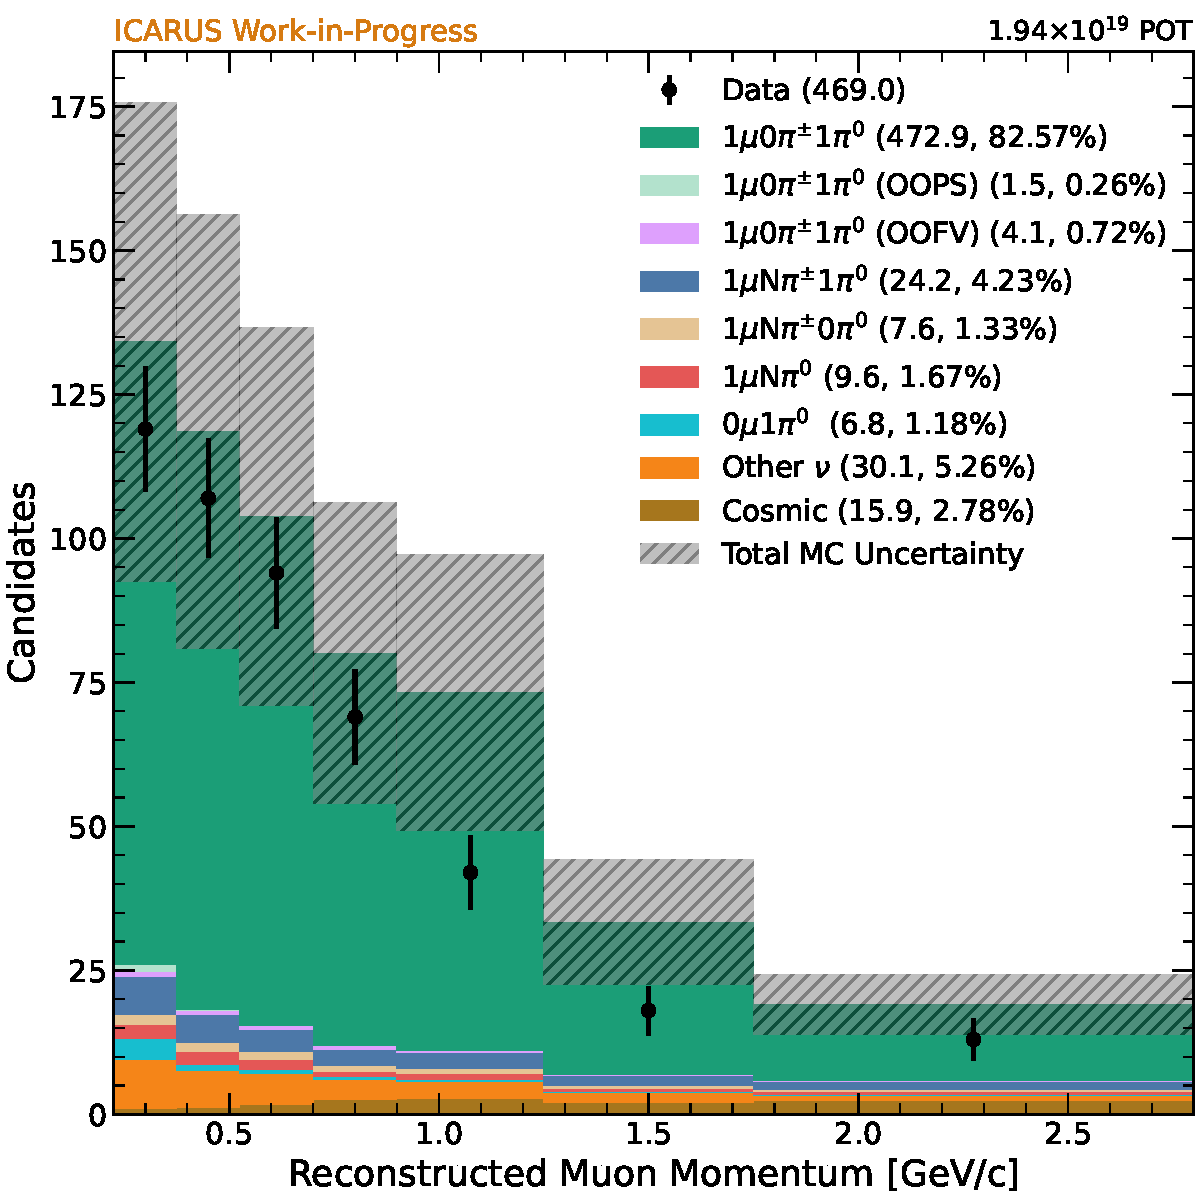
\includegraphics[width=0.50\textwidth]{reco_muon_momentum_mag_syst.pdf} \label{subfig:reco_muon_momentum_mag_syst}}
    \subfloat[Muon angle with respect to neutrino beam]
        {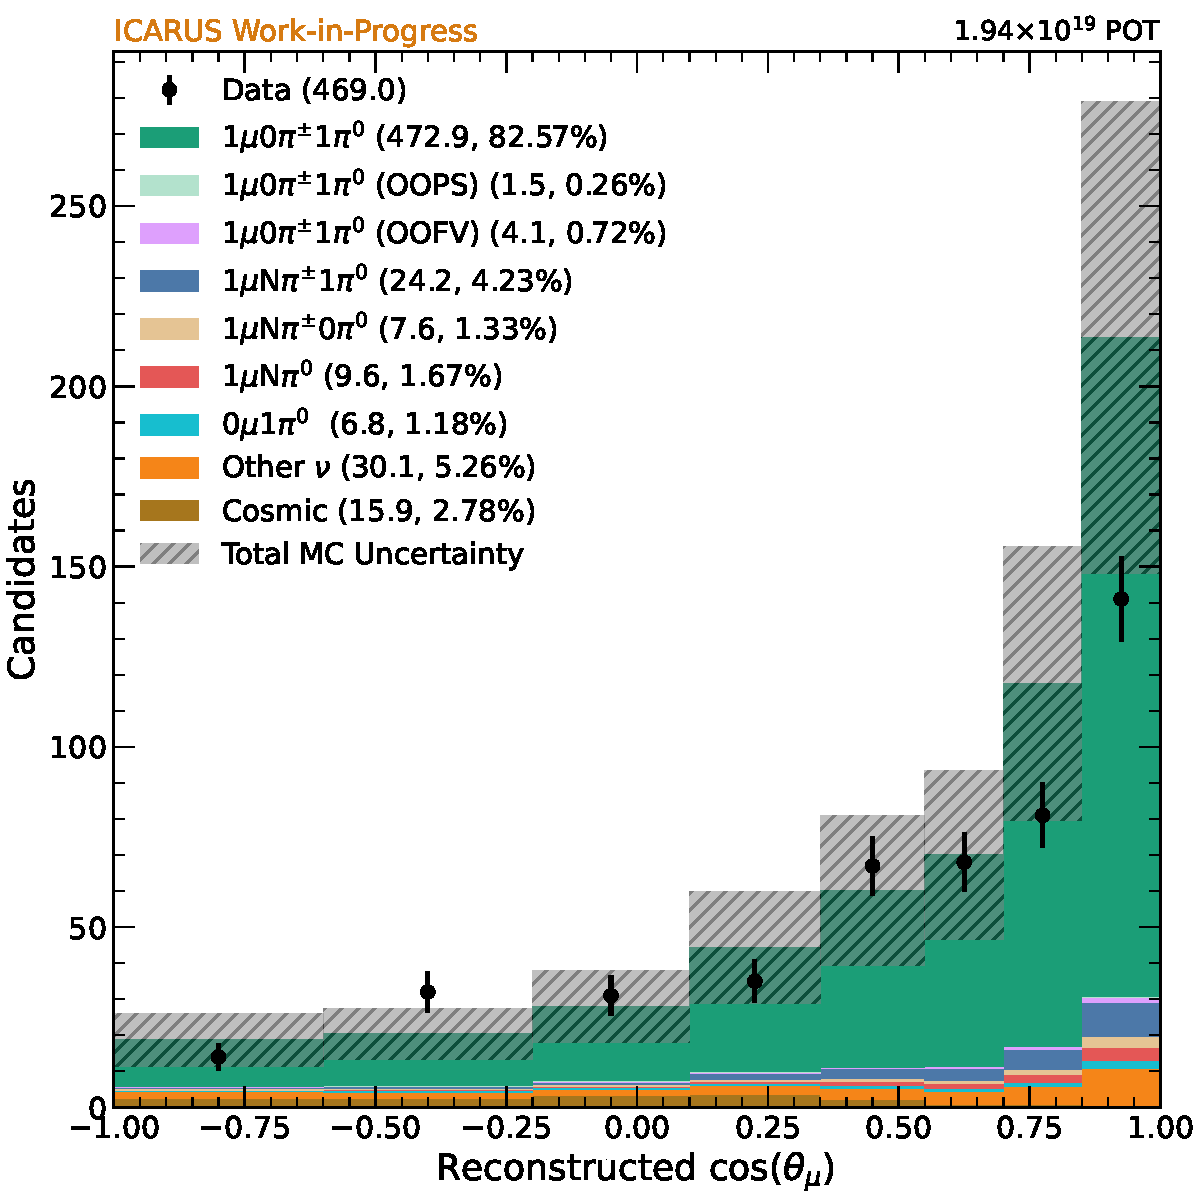
\includegraphics[width=0.50\textwidth]{reco_muon_beam_costheta_syst.pdf} \label{subfig:reco_muon_beam_costheta_syst}} \\
    \subfloat[Neutral pion momentum]
        {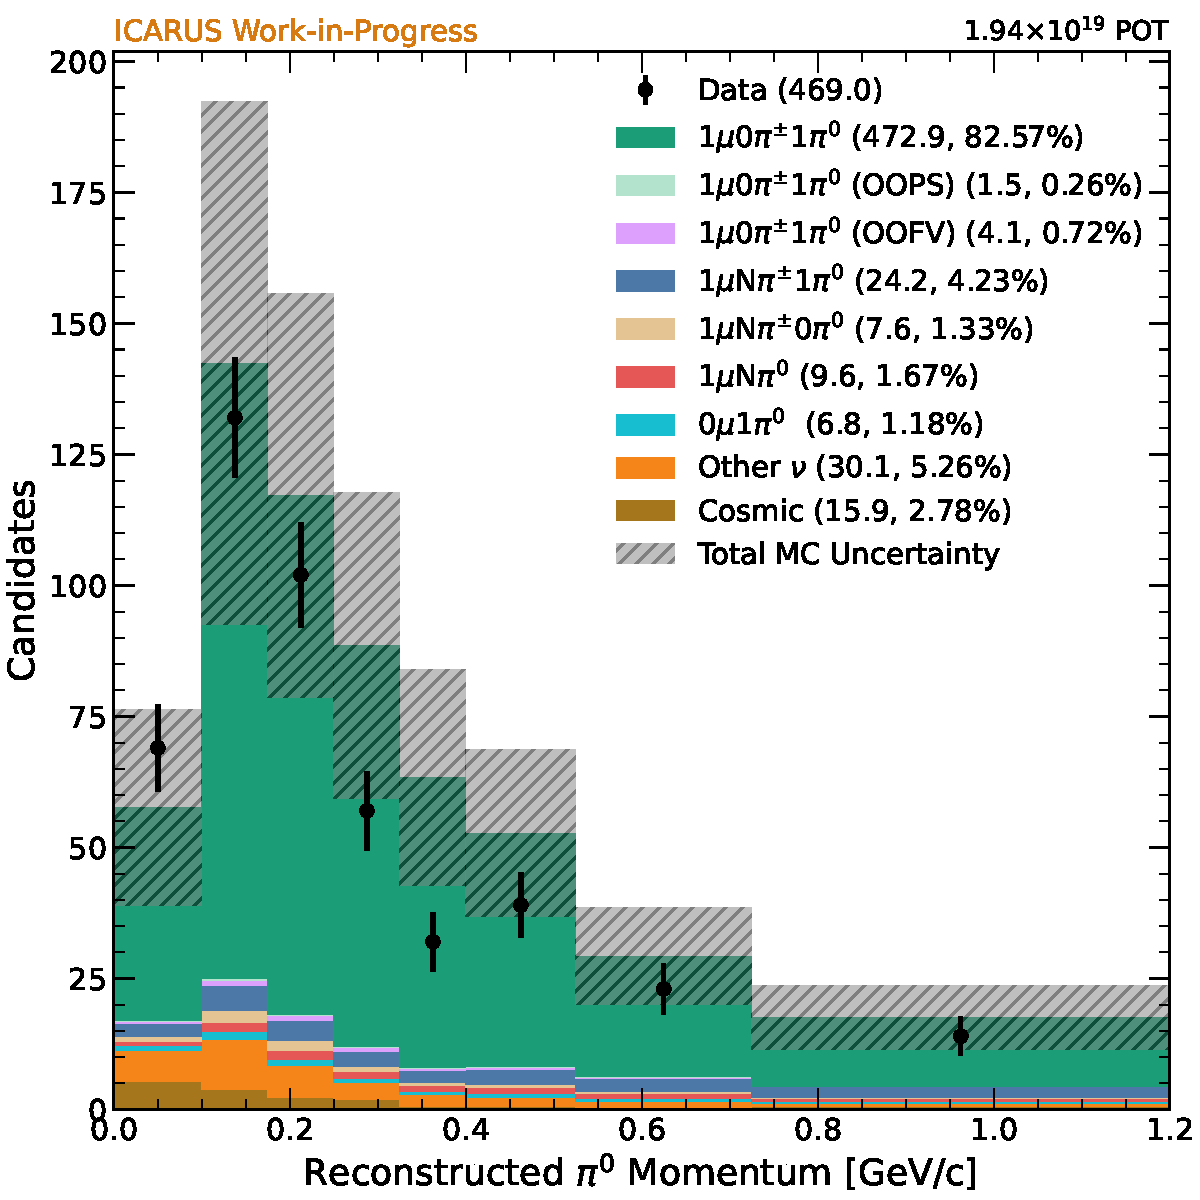
\includegraphics[width=0.50\textwidth]{reco_pi0_momentum_mag_syst.pdf} \label{subfig:reco_pi0_momentum_mag_syst}}   
    \subfloat[Neutral pion angle to neutrino beam]
        {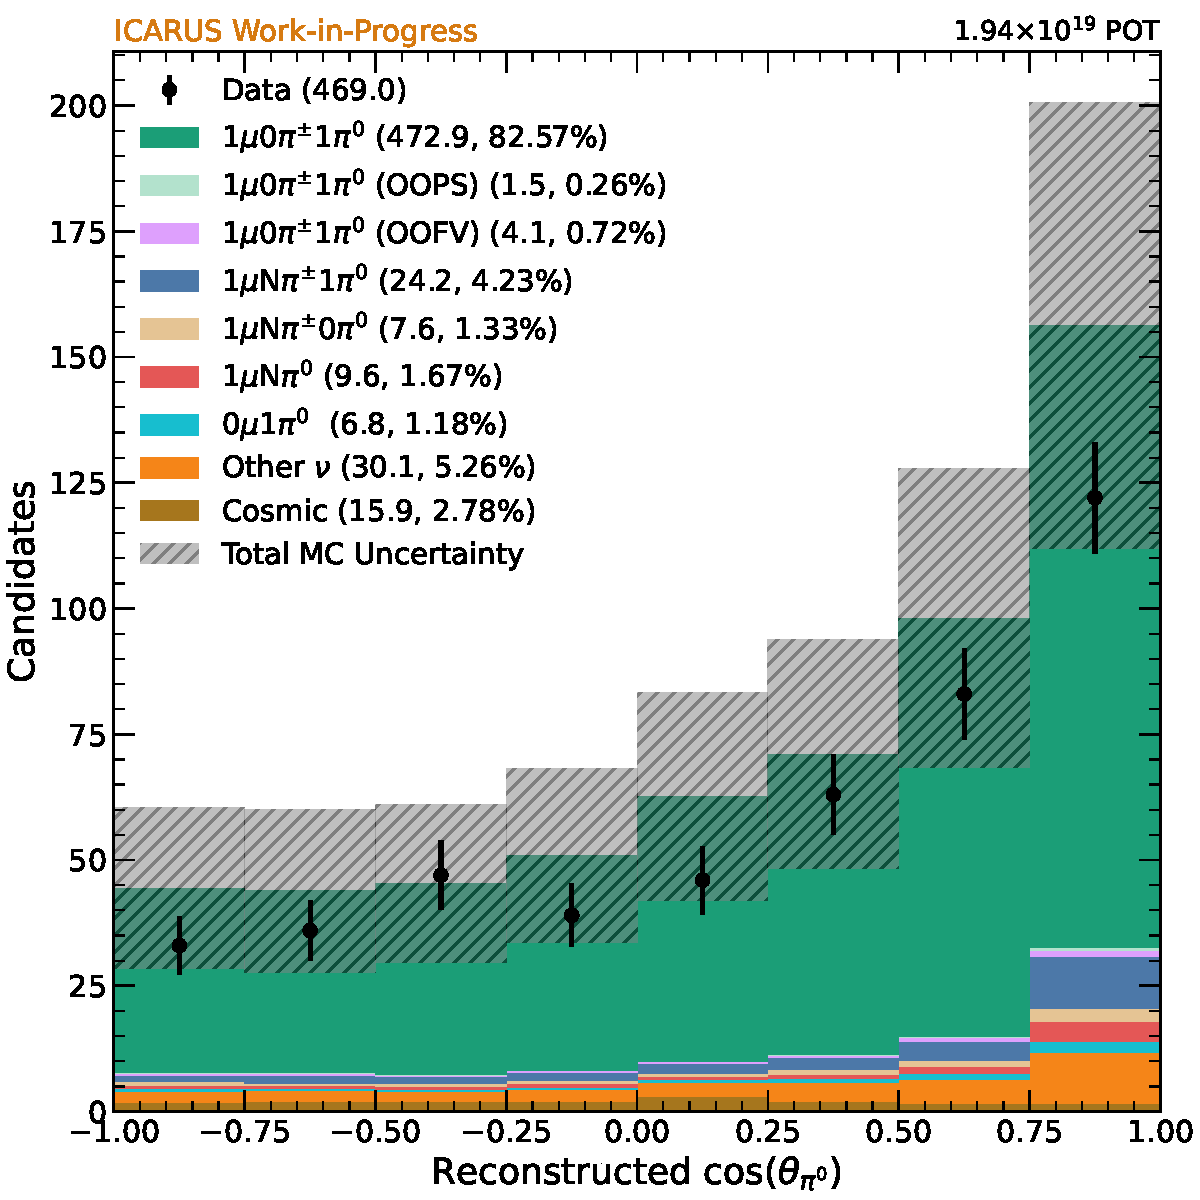
\includegraphics[width=0.50\textwidth]{reco_pi0_beam_costheta_syst.pdf} \label{subfig:reco_pi0_beam_costheta_syst}}          
    \caption{Observables chosen for analysis}
    \label{fig:reco_observables_syst}
\end{figure}

\begin{table}[H]
    \caption{Breakdown of uncertainties for $\nu_{\mu}$ CC $\pi^{0}$ selection}
    \vspace{0.1cm}
    \centering
    \begin{tabular}{ c c c } 
    \hline
    Category & Uncertainty [\%] \\
    \hline
    MC Statistical & 0.51 \\
    Offbeam Statistical & 8.64 \\ 
    Beam Flux & 8.91 \\
    Interaction Model & 30.50 \\
    Detector Response Model & 4.19 \\
    \hline
    Total & 33.0 \\
    \hline
    \end{tabular}
    \label{Tab:totaluncertainy}
\end{table}

\end{document}